
\documentclass[nooutcomes]{ximera}
%\documentclass[space,handout,nooutcomes]{ximera}

% For preamble materials

\usepackage{pgf,tikz}
\usepackage{mathrsfs}
\usetikzlibrary{arrows}
\usepackage{framed}
\usepackage{amsmath}
%\pgfplotsset{compat=1.16}

\graphicspath{
  {./}
  {algorithms/}
  {../algorithms/}
}

\pdfOnly{\renewenvironment{image}[1][]{\begin{center}}{\end{center}}}

%%% This set of code is all of our user defined commands
\newcommand{\bysame}{\mbox{\rule{3em}{.4pt}}\,}
\newcommand{\N}{\mathbb N}
\newcommand{\C}{\mathbb C}
\newcommand{\W}{\mathbb W}
\newcommand{\Z}{\mathbb Z}
\newcommand{\Q}{\mathbb Q}
\newcommand{\R}{\mathbb R}
\newcommand{\A}{\mathbb A}
\newcommand{\D}{\mathcal D}
\newcommand{\F}{\mathcal F}
\newcommand{\ph}{\varphi}
\newcommand{\ep}{\varepsilon}
\newcommand{\aph}{\alpha}
\newcommand{\QM}{\begin{center}{\huge\textbf{?}}\end{center}}

\renewcommand{\le}{\leqslant}
\renewcommand{\ge}{\geqslant}
\renewcommand{\a}{\wedge}
\renewcommand{\v}{\vee}
\renewcommand{\l}{\ell}
\newcommand{\mat}{\mathsf}
\renewcommand{\vec}{\mathbf}
\renewcommand{\subset}{\subseteq}
\renewcommand{\supset}{\supseteq}
\renewcommand{\emptyset}{\varnothing}
\newcommand{\xto}{\xrightarrow}
\renewcommand{\qedsymbol}{$\blacksquare$}
\newcommand{\bibname}{References and Further Reading}
\renewcommand{\bar}{\protect\overline}
\renewcommand{\hat}{\protect\widehat}
\renewcommand{\tilde}{\widetilde}
\newcommand{\tri}{\triangle}
\newcommand{\minipad}{\vspace{1ex}}
\newcommand{\leftexp}[2]{{\vphantom{#2}}^{#1}{#2}}

%% More user defined commands
\renewcommand{\epsilon}{\varepsilon}
\renewcommand{\theta}{\vartheta} %% only for kmath
\renewcommand{\l}{\ell}
\renewcommand{\d}{\, d}
\newcommand{\ddx}{\frac{d}{dx}}
\newcommand{\dydx}{\frac{dy}{dx}}


\usepackage{bigstrut}


\newenvironment{sectionOutcomes}{}{}

\usepackage{array}
%\setlength{\extrarowheight}{-.2cm}   % Commented out by Findell to fix table headings.  Was this for typesetting division?  
\newdimen\digitwidth
\settowidth\digitwidth{9}
\def~{\hspace{\digitwidth}}
\def\divrule#1#2{
\noalign{\moveright#1\digitwidth
\vbox{\hrule width#2\digitwidth}}}


\title{Rational Numbers}
\author{Bart Snapp and Brad Findell}
\begin{document}
\begin{abstract}
Problems about Rational Numbers.
\end{abstract}
\maketitle


%\begin{problem}
%Problem
%\begin{freeResponse}
%\begin{hint}
%Hint
%\end{hint}
%\end{freeResponse}
%\end{problem} 



\begin{problem}
Describe the set of rational numbers. Give some relevant and
  revealing examples/nonexamples.
\end{problem}

\begin{problem}
What algebraic properties do the rational numbers enjoy that the
  integers do not? Explain your reasoning.
\end{problem}

\begin{problem}
What number gives the same result when added to $1/2$ as when
  multiplied by $1/2$. Explain your reasoning.
\end{problem}

\begin{problem}
Draw a rectangle to represent a garden. Shade in $3/5$ of the
  garden. Without changing the shading, show why $3/5$ of the garden
  is the same as $12/20$ of the garden. Explain your reasoning.
\end{problem}

\begin{problem}
Shade in $2/3$ of the entire picture below:
\[
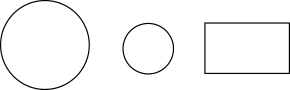
\includegraphics{fracPart.png}
\]
Explain your reasoning.
\end{problem}

\begin{problem}
What fractions could the following picture be illustrating?
\[
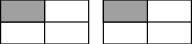
\includegraphics{whichFrac.png}
\]
Explain your reasoning.
\end{problem}

\begin{problem}
When Jesse was asked what the $7$ in the fraction $\frac{3}{7}$
  means, Jesse said that the ``$7$'' is the \textit{whole}. Explain
  why this is not completely correct. What is a better description of
  what the ``$7$'' in the fraction $\frac{3}{7}$ means?

\end{problem}



\end{document}